\documentclass[conference]{IEEEtran}
\IEEEoverridecommandlockouts

\usepackage{cite}
\usepackage{amsmath,amssymb,amsfonts}
\usepackage{algorithmic}
\usepackage{graphicx}
\usepackage{textcomp}
\usepackage{xcolor}
\usepackage[a4paper, total={184mm,239mm}]{geometry}
\def\BibTeX{{\rm B\kern-.05em{\sc i\kern-.025em b}\kern-.08em
    T\kern-.1667em\lower.7ex\hbox{E}\kern-.125emX}}
\usepackage{acronym}
\usepackage{amsmath}
\usepackage{tikz}

\usepackage{tkz-graph}

\usepackage{pgfplots}
\usetikzlibrary{arrows}

\pgfplotsset{compat=1.8}
\usepackage{filecontents}

\usepackage{mathtools}
\usepackage{mathrsfs}
\usetikzlibrary{arrows}

\usepackage{caption, subcaption}
\usepackage{comment}
\usepackage{float}

\usepackage{array}
\usepackage{tabularx}

\newenvironment{conditions*}
  {\par\vspace{\abovedisplayskip}\noindent
   \tabularx{\columnwidth}{>{$}l<{$} @{${}={}$} >{\raggedright\arraybackslash}X}}
  {\endtabularx\par\vspace{\belowdisplayskip}}

\usetikzlibrary{graphs,quotes,arrows.meta, positioning, shapes.geometric,calc}

\acrodefplural{SNN}[SNNs]{Spiking Neural Networks}

\definecolor{ududff}{rgb}{0.30196078431372547,0.30196078431372547,1.}
\definecolor{xdxdff}{rgb}{0.49019607843137253,0.49019607843137253,1.}

\usepackage{bm}
\newcommand{\param}[1]{\ensuremath{\vec{\bm{#1}}}}
% The preceding line is only needed to identify funding in the first footnote. If that is unneeded, please comment it out.
%\usepackage{cite}
%\usepackage{amsmath,amssymb,amsfonts}
%\usepackage{algorithmic}
%\usepackage{graphicx}
%\usepackage{textcomp}
%\usepackage{xcolor}
%\usepackage[a4paper, total={184mm,239mm}]{geometry}
%\def\BibTeX{{\rm B\kern-.05em{\sc i\kern-.025em b}\kern-.08em
%    T\kern-.1667em\lower.7ex\hbox{E}\kern-.125emX}}

\begin{document}

\title{A novel approach for explainable spiking neural networks\\
{\footnotesize \textsuperscript{*}Note: Sub-titles are not captured in Xplore and
should not be used}
\thanks{Identify applicable funding agency here. If none, delete this.}
}

\author{\IEEEauthorblockN{1\textsuperscript{st} Given Name Surname}
\IEEEauthorblockA{\textit{dept. name of organization (of Aff.)} \\
\textit{name of organization (of Aff.)}\\
City, Country \\
email address or ORCID}
\and
\IEEEauthorblockN{2\textsuperscript{nd} Given Name Surname}
\IEEEauthorblockA{\textit{dept. name of organization (of Aff.)} \\
\textit{name of organization (of Aff.)}\\
City, Country \\
email address or ORCID}
\and
\IEEEauthorblockN{3\textsuperscript{rd} Given Name Surname}
\IEEEauthorblockA{\textit{dept. name of organization (of Aff.)} \\
\textit{name of organization (of Aff.)}\\
City, Country \\
email address or ORCID}
\and
\IEEEauthorblockN{4\textsuperscript{th} Given Name Surname}
\IEEEauthorblockA{\textit{dept. name of organization (of Aff.)} \\
\textit{name of organization (of Aff.)}\\
City, Country \\
email address or ORCID}
\and
\IEEEauthorblockN{5\textsuperscript{th} Given Name Surname}
\IEEEauthorblockA{\textit{dept. name of organization (of Aff.)} \\
\textit{name of organization (of Aff.)}\\
City, Country \\
email address or ORCID}
\and
\IEEEauthorblockN{6\textsuperscript{th} Given Name Surname}
\IEEEauthorblockA{\textit{dept. name of organization (of Aff.)} \\
\textit{name of organization (of Aff.)}\\
City, Country \\
email address or ORCID}
}

\maketitle

\begin{abstract}
Spiking Neural Networks (SNN) are the third generation of Artificial Neural Networks (ANNs) that are considered 
more efficient, and potentially more expressive, than conventional AI models. Similar to the current ANNs, the outputs of SNNs are not interpretable and the behavior of the model is not comprehended, hence SNNs are considered as black boxes.
Moreover, current verification methods for SNNs focus on modelling the behaviour of each individual neuron, hence they are not scalable especially when
the number of neurons in the system grows, limiting their use in safety-critical applications.
    
In this paper, we introduce methods to model an SNN-based
system as a set of transfer functions that capture the behaviour
of each group of neurons. We use Fourier transform to extract the
fundamental neuron behaviour from their noisy, spiking outputs. 
The transfer function is then derived to capture the behaviour of the overall SNN, 
and the system is reconstructed using computational blocks that capture these transfer functions. 
Safety-critical properties are then verified over this transfer function model using the model checker SPIN.
This work allows to express the behavior of SNNs as transfer functions to explain how the outputs of the model are derived over the range of inputs.
Furthermore, it provides methods to verify an SNN-based system, regardless of the number of neurons, using tools and techniques to abstract the network behaviour.
\end{abstract}

\begin{IEEEkeywords}
component, formatting, style, styling, insert
\end{IEEEkeywords}

\section{Introduction}
The human brain is the most efficient computing unit since the existence of mankind.
The biological organ, which has a volume of about 1300 cubit centimeter, can processes and memorizes tremendous amount of information with
a fraction of energy compared to the conventional electrical computing systems. One of the most powerful supercomputers in the world has been
recently demonstrated to require a million times more power, 20 megawatts, to compute the mathematical operations that the human brain could compute 
with just 20 watts of energy (numenta).

With the recent advance in Artificial Intelligence (AI), there has been many successful applications to develop an electrical system to mimic the 
characteristics of the human brain. The conventional Artificial Neural Networks (ANNs), such as Multi-Layer Perceptrons (MLPs) and Convolutional Neural Networks (CNNs) are all shown to be able to achieve
some level of success to mimic the behavior of the human brain (mediaMIT). However, the energy efficiencies of all these models are significantly lacking compared to the human brain. 
For example, ChatGPT-3, which is a human-like chatbox that uses the structure of MLP, is estimated to consume 935MWh 
of power, which is approximately the same energy used by 30,632 US households per day (numenta).
Moreover, the conventional AI systems are often hard to be deployed on the edge devices due to their high energy consumption.

A spiking neural network (SNN) (ghosh2009spiking) is an artificial neural network that is more plausiable to the biological neuron than the conventional ANNs. In SNNs, neurons
communicate with each other using spikes through synapses connecting the neurons where the synapses has the trainable weight values that decodes the spikes to the real value. Since the information is carried with a train of spikes, it naturally
operates in temporally sparse activity, enabling event-driven computing. This allows the SNN to be far more efficient than the conventional ANNs as the output is decoded only
when the spike is received. However, the discrete and discontinuity of the spiking signal causes the
difficulty to apply the backpropagation algorithm to train the neural network. Hence, it is broadly accepted that SNNs are less accurate than the conventional ANNs.

In this paper, we provide methods to explain the properties of already trained SNNs and be able to verify the
system to guarantee the verification properties. Hence, the users can guarantee that the trained SNNs are accurate enough to be used for their application.
\section{Background-Leaky Integrate and Fire}

Respiratory Sinus Arrhythmia (RSA) is the natural modulation in heart rate synchronized to breathing. It is characterized by an increase in heart rate during inspiration and a decrease during expiration.  It is the beneficial arrhythmia observed strongly on healthy individuals while its presence diminishes on the  patients with Heart Failure. Although the fundamental reason for the existence of RSA is still debatable, recent studies show that RSA increases the efficiency of cardiac output. Hence, it gives rise to the hypothesis that restoring RSA could bring therapeutic benefits to the patients. 

Implantable medical devices, such as a pacemaker have many constraints, that need to be considered before they are installed in the human body. Their functional correctness needs to be guaranteed as it is directly related to the safety of the patient. The size needs to be small enough, and the energy efficiency needs to be high. Hence, the simplicity of the structure is the key factor to be considered.

A human heart is a natural pacemaker driven by the intricate workings of the nervous system. Sympathetic and parasympathetic nerves are part of the autonomic nervous system, which regulates the involuntary body functions like heart rate and the respiratory rate. The heart is driven by neurons, hence it may be beneficial to use neural model for the pacemaker mechanism.

Neurons are fundamental building blocks of the nervous system that control various functions throughout the body. When the internal membrane voltage of the neuron reaches a certain threshold, it triggers the generation of a voltage spike. This voltage spike propagates to the neighboring neurons, which integrates their membrane voltages for the generation of the spikes for their neighboring neurons. Hence, the information is encoded by the frequency and the magnitude of the spiking signal. 

The LIF model is a simplified mathematical model that mimics the behavior of individual neurons. In the LIF neuron, the received input, which is often referred as an input current, integrates the internal membrane voltage. When the membrane voltage reaches a certain threshold, a spike is created and the membrane voltage resets to zero. Once the spike is generated, the neuron enters the resting mode for the refractory period during which the membrane voltage stays zero regardless of the input.


\begin{figure}[htbp]
	\centerline{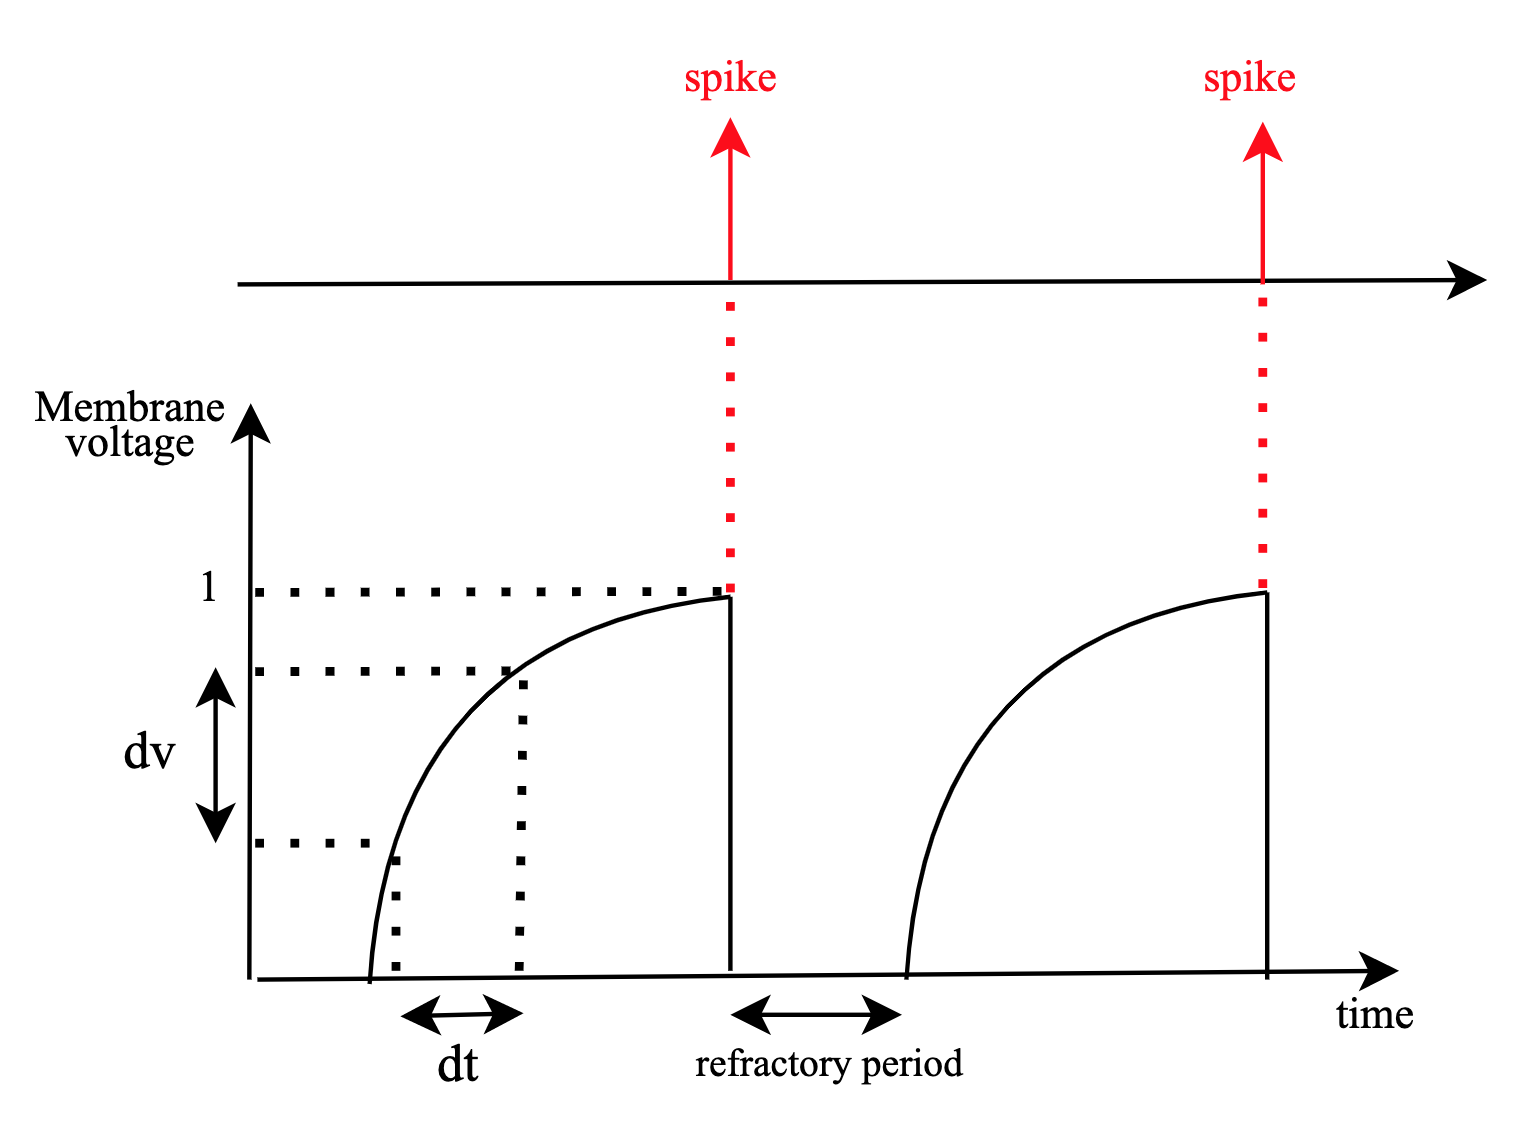
\includegraphics[scale=0.25]{./fig/lif.png}}
	\caption{LIF neuron model.}
	\label{lif}
\end{figure}



The following formula determines the membrane voltage of an LIF neuron:
\begin{equation} \label{lifneuron}
	dv = (I_i - v) \times (1 - e^{-dt/RC})
\end{equation}

where:
\begin{conditions*}
	dv     &   change in the membrane voltage \\
	
	v     &   current membrane voltage \\
	
	dt     &   time step  \\
	
	RC    &   membrane time constant
\end{conditions*}


Once the membrane voltage reaches the threshold value of 1, a spike is generated and the refractory period follows. During the refractory period, the membrane voltage stays 0 regardless of the input current.


\section{Methodology}

In this section, we illustrates how to determine each parameter of the LIF neuron to function as a  RSA pacemaker.

\begin{figure}[htbp]
	\centerline{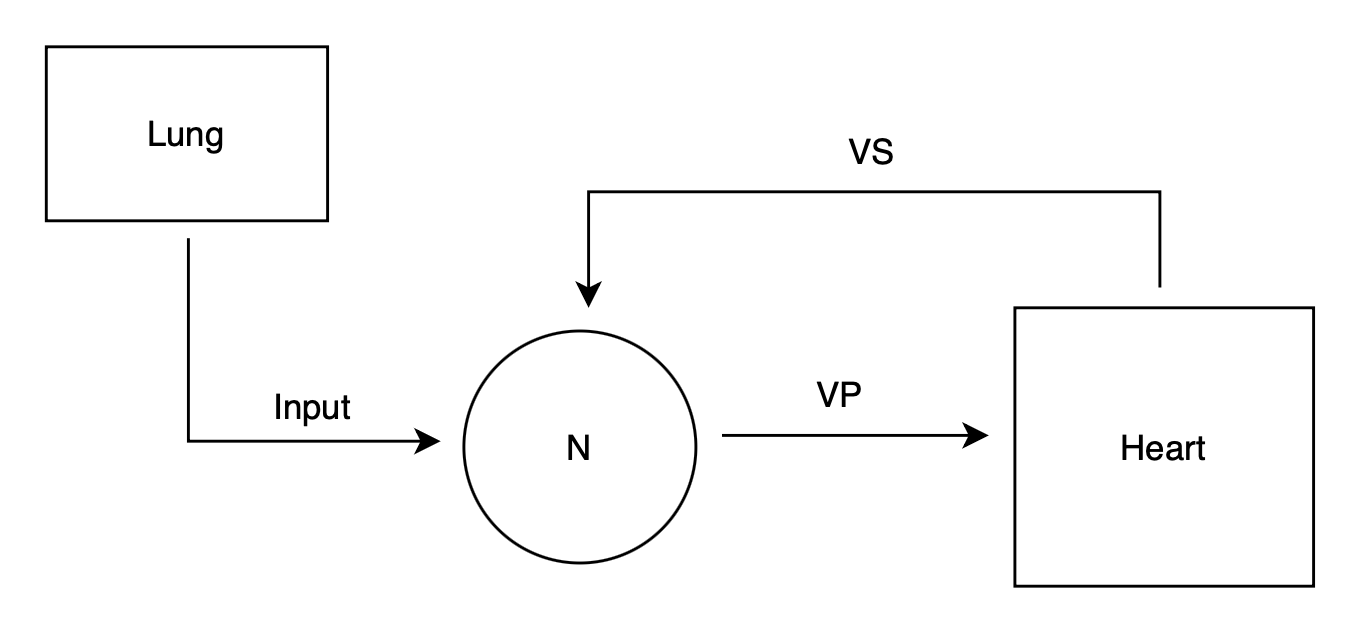
\includegraphics[scale=0.25]{./fig/overall.png}}
	\caption{Overall structure of RSA pacemaker.}
	\label{lif}
\end{figure}

The pacemaker is constructed as a single chamber ventricular mode. It receives two inputs, one from the lung and one from the heart. The signal from the lung is a square wave with the high period meaning the inspiration and the low period meaning the expiration. This signal is used as an input for the neuron to control the frequency of the spike.  The spike generated from the LIF neuron is used as a Ventricular Pacing (VP) to stimulate the heart. The neuron also reads the ventricular signal from the heart, ventricular sense (VS), to monitor the natural heart beat of the heart.

From equation (1), the time for the membrane voltage to reach the threshold voltage 1 is:



\section{Result}
The pacemaker was tested with a virtual heart and a lung. The virtual heart is programmed to produce a ventricular signal with the frequency that is set. The virtual lung gives the respiratory signal which is the periodic square wave.

To test if the RSA pacemaker can operate as a basic pacemaker, the 


\begin{figure}[htbp]
	\centerline{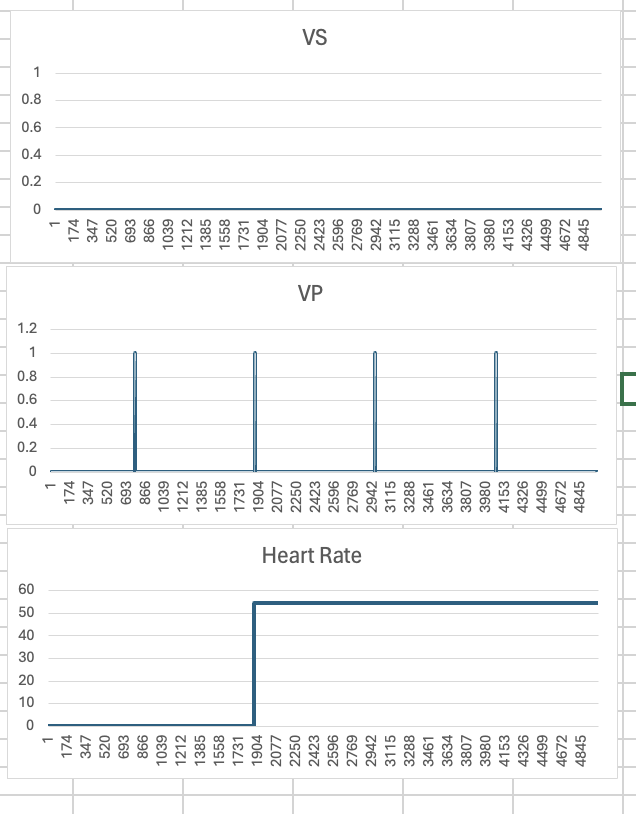
\includegraphics[scale=0.5]{./fig/result_dead.png}}
	\caption{Results with dead heart.}
	\label{lif}
\end{figure}


\begin{figure}[htbp]
	\centerline{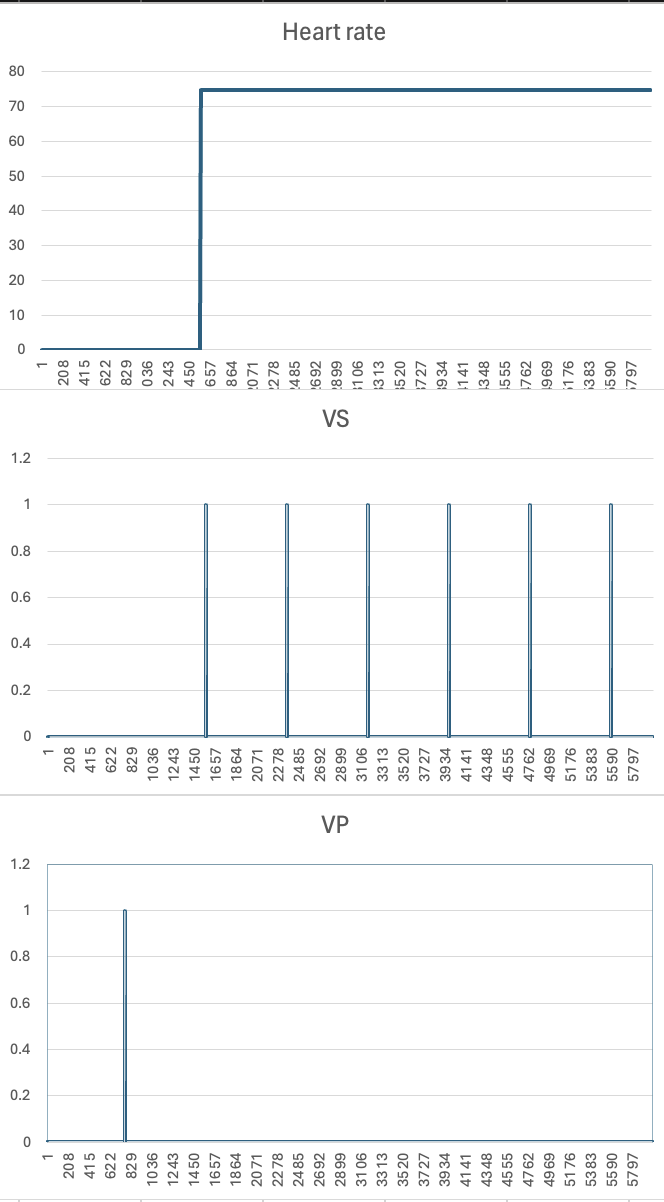
\includegraphics[scale=0.5]{./fig/result_75.png}}
	\caption{Virtual heart set to 75bpm RSA off Mimum heart rate set to 55.}
	\label{lif}
\end{figure}

\begin{figure}[htbp]
	\centerline{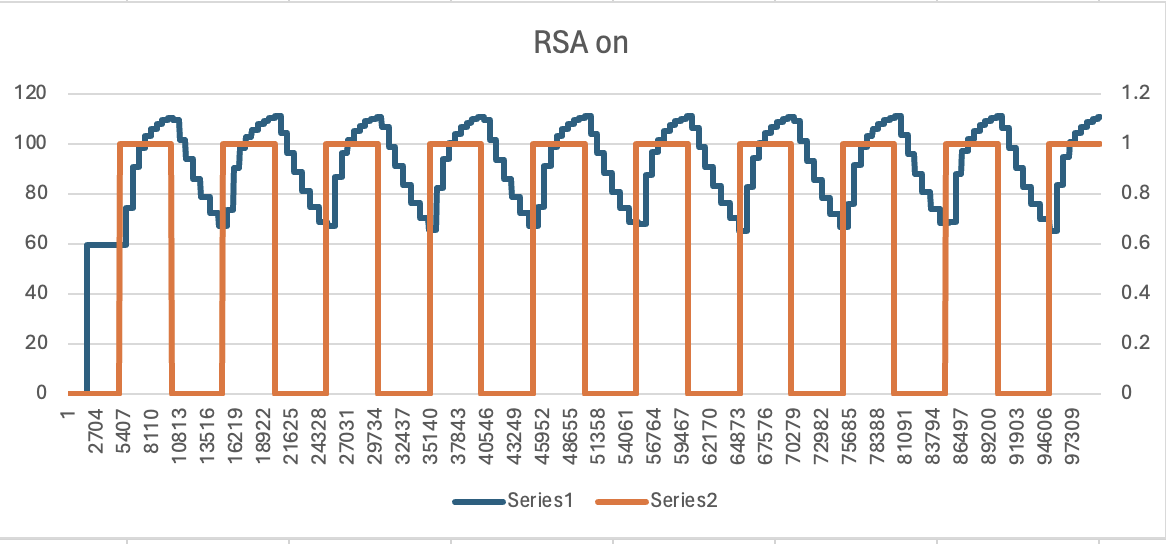
\includegraphics[scale=0.5]{./fig/result_rsa.png}}
	\caption{RSA between min to max}
	\label{lif}
\end{figure}

\begin{figure}[htbp]
	\centerline{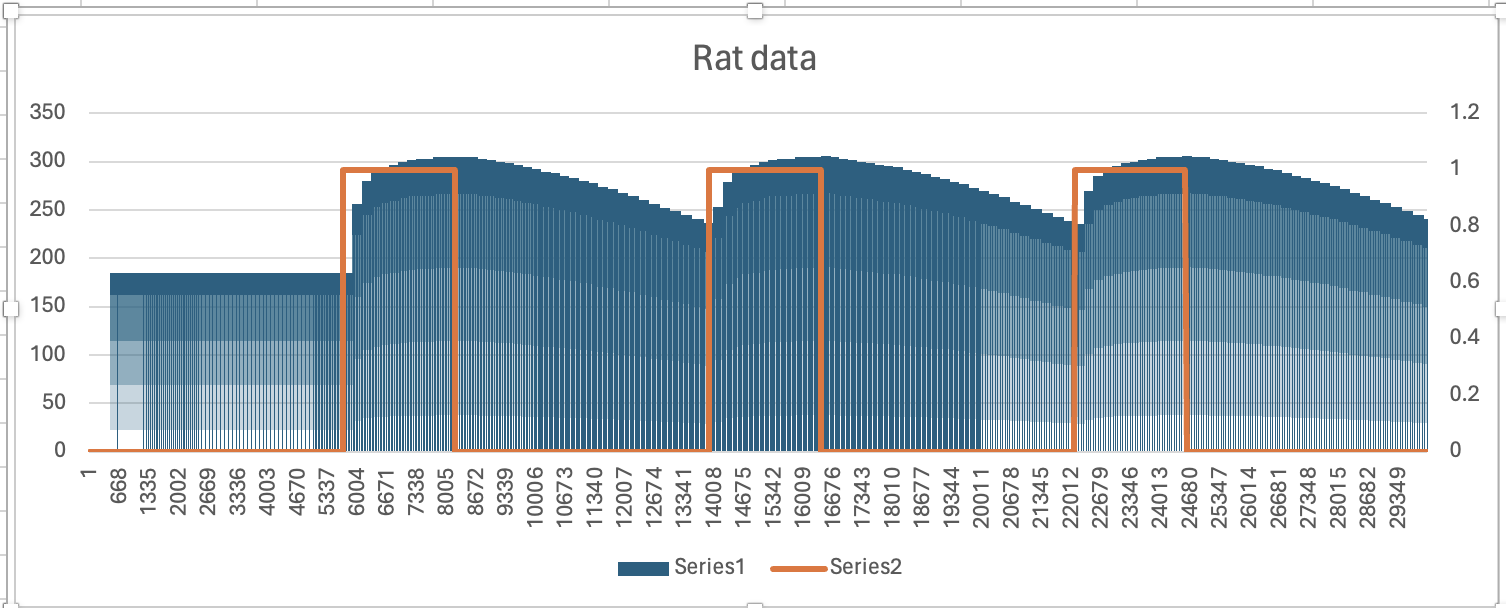
\includegraphics[scale=0.5]{./fig/result_rat.png}}
	\caption{RSA between min to max}
	\label{lif}
\end{figure}




\end{document}
